% !TeX encoding = UTF-8
% !TeX spellcheck = sv_SE

\chapter{Teknik}

I teknikkapitlet kommer vi titta på en mängd begrepp som har med radioteknik
att göra. Det är effekt och brus, beräkning av radiohorisont och utbredning
och mycket mer i detta kapitel som kan vara till nytta för radiooperatören att
känna till.

\clearpage

\section{Decibel}

Decibel är ett grundläggande begrepp inom radiovärlden och är i grunden en
logaritmisk skala som bygger på tiologaritmen. Från början använde man
begreppet Bel [B] (efter Alexander Graham Bell) men det blir ofta decimaltal
så i stället så kör man decibel. Det går 10 dB på 1 B.

Definitionen på decibel är enligt följande:

\begin{equation}
  \text{dB} = 10 \cdot \log_{10} \left( \frac{P_{ut}}{P_{in}} \right)
\end{equation}

där dB är antalet decibel, $P_{up}$ är effekten som kommer ut ur något och
$P_{in}$ är effekten som går in. Detta något kan vara en förstärkare, en
dämpare, en kabel eller nästan vad som helst som radiosignalen går igenom.

Som minnesregel kan man minnas att +3 dB betyder att effekten dubblats. Om vi
matar in 10 W i en förstärkare och får ut 20 W är förstärkningen 3 dB. På
samma sätt är -3 dB en förlust av 50 \% så om vi har en kabel med förlusten 3
dB för en viss frekvens så tappar vi halva effekten i kabeln.

\begin{table}[h]
\centering
\begin{tabular}{rr|rr|rr|rr}
	\bf dB & \bf faktor & \bf dB & \bf faktor & \bf dB & \bf faktor & \bf dB & \bf faktor \\ \hline
	     1 &       1,26 &     10 &         10 &     -1 &       0,79 &    -10 &        0,1 \\
	     2 &       1,58 &     20 &        100 &     -2 &       0,63 &    -20 &       0,01 \\
	     3 &       2,00 &     30 &     1\,000 &     -3 &       0,50 &    -30 &      0,001 \\
	     5 &       3,16 &     50 &   100\,000 &     -5 &       0,32 &    -50 &  0,000\,01
\end{tabular}
\caption{Decibel och omräkningsfaktorer}
\end{table}

\subsection{Effekt i dBW och dBm}

Effekter anges i W eller i decibel relaterat till 1 mW (dBm) eller relaterat
1W (dBW). Tabell över effekt och decibelwatt nedan:

\begin{table}[H]
\centering
\begin{tabular}{rrr|rrr|rrr}
	\textbf{Effekt} & \textbf{dBW} & \textbf{dBm} & \textbf{Effekt} & \textbf{dBW} & \textbf{dBm} & \textbf{Effekt} & \textbf{dBW} & \textbf{dBm} \\ \hline
	    1 \textmu W &          -60 &          -30 &             1 W &            0 &           30 &           100 W &           20 &           50 \\
	   10 \textmu W &          -50 &          -20 &             3 W &            5 &           35 &           250 W &           24 &           54 \\
	  100 \textmu W &          -40 &          -10 &             5 W &            7 &           37 &           500 W &           27 &           57 \\
	           1 mW &          -30 &            0 &            10 W &           10 &           40 &            1 kW &           30 &           60 \\
	          10 mW &          -20 &           10 &            20 W &           13 &           43 &          1.5 kW &           32 &           62 \\
	         100 mW &          -10 &           20 &            50 W &           17 &           47 &          2.0 kW &           33 &           63
\end{tabular}
\caption{Tabell över effekt och dBW/dBm}
\end{table}

\subsection{Antennvinst i dBi och dBd}

Riktantenner sägs ha en så kallad antennvinst och den berättar något om
antennens riktverkan. En riktantenn har en (eller några få) riktningar som den
fungerar mycket bra i, övriga riktningar är den sämre än en rundstrålande
antenn.

En rundstrålande antenn strålar lika mycket i alla riktningar i ett plan.
Detta gäller exempelvis en vertikalt monterad dipol eller kvartsvågsantenn på
ett jordplan.

Antennvinsten kan jämföras med en vanlig dipol och då använder man begreppet
dBd där den sista bokstaven står för "jämfört med en dipolantenn". I
professionella radiosammanhang använder man dock en tänkt teoretisk antenn som
strålar exakt likadant i alla riktningar, inte bara i planet utan även uppåt
och nedåt. En sådan antenn finns egentligen bara i teorin men gör det möjligt
att skapa ett referensmått för just riktverkan, denna teoretiska antenn kallas
för "isotrop antenn" och då använder man beteckningen dBi där i på slutet står
för just isotrop antenn.

Skillnaden i de båda måtten kan räknas om enligt följande:

\begin{align}
\text{dBi} &= \text{dBd} + 2,15\\
\text{dBd} &= \text{dBi} - 2,15
\end{align}

\section{S-värden, signalvärde, S-meter}

Signalstyrkan i amatörradio uttrycks oftast som S-värden. Dessa fås i regel
genom nivån på AGC hos mottagaren. Därför ser man sällan utslag vid riktigt
låga signaler.

Standard kalibrering för S-metern är enligt skalan i tabellen
\ref{tab:s-varden}. Som syns kalibreras tabellen olika för om man är under
30\,MHz (kortvåg och lägre frekvenser) och skillnaden är 20\,dB med högre
känslighet över 30\,MHz dvs VHF och uppåt.


\begin{table}[ht]
\centering
\begin{tabular}{r|rr|rr||r|rr|rr}
      & \multicolumn{2}{c|}{\textbf{$<$ 30 MHz}} &
  \multicolumn{2}{c}{\textbf{$>$ 30 MHz}}       && \multicolumn{2}{c|}{\textbf{$<$ 30 MHz}} &
  \multicolumn{2}{c}{\textbf{$>$ 30 MHz}}\\ \textbf{S} & \textbf{dBm}
  & \textbf{\textmu V} & \textbf{dBm} & \textbf{\textmu V}&   \textbf{S} & \textbf{dBm}
  & \textbf{\textmu V} & \textbf{dBm} & \textbf{\textmu V} \\\hline

	   1 & -121 & 0.21  & -141 & 0.02 & 9+10 & -63 & 160  & -83 & 16  \\
	   2 & -115 & 0.40  & -135 & 0.04 & 9+20 & -53 & 500  & -73 & 50  \\
	   3 & -109 & 0.80  & -129 & 0.08 & 9+30 & -43 & 1600 & -63 & 160 \\
	   4 & -103 & 1.60  & -123 & 0.16 & 9+40 & -33 & 5000 & -53 & 500 \\
	   5 & -97  & 3.20  & -117 & 0.32 &      &     &      &     &     \\
	   6 & -91  & 6.30  & -111 & 0.63 &      &     &      &     &     \\
	   7 & -85  & 12.60 & -105 & 1.26 &      &     &      &     &     \\
	   8 & -79  & 25.00 & -99  & 2.50 &      &     &      &     &     \\
	   9 & -73  & 50.00 & -93  & 5.00 &      &     &      &     &     \\
\end{tabular}
\caption{Tabell över S-värden, effekt och spänning}
\label{tab:s-varden}
\end{table}

\section{Modulationer}

\subsection{Bandbredd olika modulationer}

Olika modulationer upptar olika bandbredd. Detta är mycket viktigt att förstå
när man ställer in sin radiostation. Detta gäller särskilt att beakta i
närheten av nödfrekvenser eller bandkanten. När vi talar om bandbredder här
förstås den bandbredd vari minst 98\% av signalens effekt befinner sig.

\begin{table}[H]
\centering
\begin{tabular}{lrl}
	\textbf{Modulation} & \textbf{Bandbredd} & \textbf{Kommentarer}                  \\ \hline
	CW                  &          $<$500 Hz & Smalbandigt                           \\
	AM                  &              6 kHz & Amplitudmodulering med fullt sidband  \\
	SSB*                &              <3 kHz & Amplitudmodulering med enkelt sidband \\
	NFM                 &           7-12 kHz & Smalbandig FM                         \\
	FM                  &             16 kHz & Normal FM                             \\
	WFM                 &          16-75 kHz & Bredbandig FM (t.ex. rundradio)
\end{tabular}
\caption{Normal bandbredd vid olika modulationsslag}
\end{table}

För SSB gäller att USB och LSB fungerar lite olika. När man beräknar den
högsta eller lägsta frekvensen utgår man från den inställda frekvensen $f$.
För USB gäller då att högsta frekvensen är $f+3$\,kHz. För LSB blir det
$f-3$\,kHz. Detta innebär att om du sänder på 80\,m-bandet och du får sända
telefoni från 3600--3800\,kHz och vill lägga dig i undre bandkanten och köra
LSB skall du ställa in din radio på 3603\,kHz som lägsta frekvens. Använd
gärna lite marginal och kör exempelvis 3605\,kHz i stället.

Den egentliga modulationsfrekvensen är dock lite mer komplicerad. Normalt
anges den verkliga modulationsfrekvensen som ca 2,7\,kHz och det beror på att
man i regel filtrerar bort ljudet under 300\,Hz och det över 3000\,Hz. Detta
innebär att det akustiska frekvensomfånget blir 300--3000\,Hz och därmed
upptar signalen inte mer än 2,7\,kHz.

Det är vanligt att man märker stationer som kör överdriven bandbredd. Antingen
som en följd av att man vill öka sin modulationsvinst, okunskap eller man har
skruvat i sin radio. Syftet kan var att få bättre genomslag vid långväga
förbindelser.

\subsection{Telegrafi, CW}

CW står för continuous waves och innebär en rent omodulerad bärvåg. I
mottagaren används en oscillator för att återskapa hörbar signal. Detta
används för telegrafi och modulationsslaget är oftast A1A. Ibland sänds
telegrafi som modulerad AM-bärvåg också som då moduleras med t.ex. 700\,Hz
ton. Det är dock mindre vanligt.

Bandbredden för CW är i teorin mycket smal. I praktiken blir den lite beroende
på frekvens från några Hz till något hundratal Hz beroende på frekvensband och
sändarens beskaffenhet i form av jitter och frekvensstabilitet.

Bandbredden hos CW består av fasbruset vilket normalt är så undertryckt att det
egentligen inte betyder så mycker samt stig- respektive falltiden när man
nycklar eller släpper nyckeln. Sker detta mjukt är bandbredden låg, har man
skarp in- eller urkoppling av bärvågen nyttjar man mer bandbredd.

\subsection{Amplitudmodulering, AM}

Amplitudmodulering finns i flera olika varianter. Vanlig AM består av en
bärvåg vars styrka varieras i takt med signalen som skall sändas. Denna
förändring av bärvågen producerar sidband och det är i dessa som den egentliga
informationen återfinns. Bärvågen i sig får dock lejonparten av signalen
varför det är en sändningsklass som nästan aldrig används inom
amatörradiobanden.

Bandbredden hos AM-modulerad signal kan beräknas genom att man tar två gånger
högsta modulationsfrekvensen. Detta ger t.ex. vid en modulationsfrekvens som
går från 300-3000\,Hz en bandbredd som varierar med talet från upp till
6\,kHz.

\begin{equation}
	B=2f_m
\end{equation}

Där $f_m$ är högsta modulationsfrekvensen.

\subsection{SSB/ESB -- Enkelt sidband, en AM-variant}

Enkelt sidband används av radioamatörer för att minska på bandbredden samt
lägga radioenergin där den behövs mest. Eftersom båda sidbanden innehåller
samma information kan man filtrera bort dessa samt bärvågen innan man matar
sändarens förstärkarsteg med resultatet. I mottagaren behöver man dock
återskapa en referenssignal, en så kallad beat-oscillator gör detta. När man
ställer in frekvensen så försöker man därmed matcha den ursprungliga
frekvensen. Ligger man för långt från låter det kalle anka, kommer man för
nära sidbandet låter det dovt och basigt.

Enkelt sidband förkortas ESB eller SSB (single side-band) och man kan välja
vilket sidband man vill använda sig av. På amatörradiofrekvenser under 10 MHz
använder man LSB (lägre/lower sidbandet) och på frekvenser över 10 MHz används
USB/ÖSB (upper/övre sidbandet).

Detta är mycket av tradition. Använder man fel sorts sidband hörs det inget
vettigt när man försöker lyssna. Språkrytmerna gör dock att vi uppfattar det
som att mänskligt tal förekommer. I dag händer det att amatörer bryter mot
regeln och sänder med ``fel'' sidband på fel frekvens.

Bandbredden hos SSB är halva den för normal AM egentligen. Den kan därmed
beräknas som för AM och halveras.

\begin{equation}
	B=f_m
\end{equation}

Där $f_m$ är högsta modulationsfrekvensen.

\subsection{Frekvensmodulering, FM}

Frekvensmodulering består av att man tar en bärvåg och modulerar den med talet
genom att skifta dess frekvens. Om skiftet i frekvens är mycket litet kallas
moduleringen för fasmodulation. FM-modulering indelas i lite olika klasser
beroende på hur stor deviation som används. På amatörradions VHF- och UHF-band
talar vi om FM och NFM (Narrow FM, andra namn förekommer också). Ibland talar
man om bred FM, normal FM och smal FM på svenska.

Normal FM innebär att deviationen (hur mycket signalen avviker från
grundfrekvensen) är lika stor som den högsta modulationsfrekvensen. Det är
vanligt att kommunikationsradio använder sig av 3 kHz som högsta
modulationsfrekvens och 5 kHz deviation. Deviationen är då något bredare och ger
upphov till en viss modulationsvinst. När man talar om FM-radio på UKV-bandet
för rundradio så är deviationen ca 75\,kHz och högsta modulationsfrekvens ca
16\,kHz. Där är alltså svinget betydligt bredare än modulationen och detta är
bred FM.

Nu för tiden förordas en minskning av bandbredden för FM-sändningar på
amatörbanden, främst är det väl VHF och UHF där FM-sändning är vanligast
förekommande och där vill man ha en kanalindelning om 12,5\,kHz i stället för
som tidigare 25\,kHz. Om man studerar bandbredden hos olika FM-signaler kan
man använda sig av Carsons bandbreddsbegrepp:

\begin{equation}
	B=2(f_M+f_D)
\end{equation}

Där $B$ är bandbredden $f_M$ högsta modulationsfrekvensen och $f_d$ är
FM-signalens maximala deviation (även kallat sving). Carsons bandbreddsbegrepp
säger att 98\% av energin förekommer inom den stipulerade bandbredden. Det
betyder att att grannkanalen kan få ungefär 17\,dB lägre signal under sändning
vilket fortfarande inte är enormt bra. Carson var för övrigt den som faktiskt
uppfan SSB-modulationen.

\begin{center}
\begin{tabular}{rrrr}
	Deviation & Modulation & Bandbredd & Kanaldelning \\ \hline
	    5 kHz &      3 kHz &    16 kHz &       25 kHz \\
	  2.5 kHz &      3 kHz &    11 kHz &     12.5 kHz
\end{tabular}
\end{center}

\section{Vågutbredning}
\label{vågutbredning}
\index{vågutbredning}

Vågutbredning är något som är väldigt viktigt för radiokommunikation och
beroende på vilken frekvens som används kan vågutbredningen se mycket olika ut
för olika radiosändningar. För VHF och uppåt är det i princip bara markvåg men
för lägre frekvenser kan också rymdvågsutbredning ske.

\subsection{Markvåg}
\index{markvåg}

Markvågen är den vanligaste radioutbredningen vi tänker oss, här får man hjälp
av att placera antennan över terrängen och på hustak för att få så fri sik som
möjligt vilket ökar längden på markvågsutbredningen. Det är också den
utbredning som handhållna radioapparater nyttjar men i och med att man som
regel då kommer vara mycket nära marken blir oftast utbredningen begränsad.

I närheten av vatten kan markvågen ofta gå längre än till lands. Det är mindre
saker som hindrar den och skillnaden i vattnets och luftens dielektricitet gör
att radiosignalen kan följa ytan lite längre innan den klingat av.

\subsection{Rymdvåg}
\index{rymdvåg}

Rymdvåg är något som framför allt uppträder på kortvåg. När strålningen från
solen träffar de övre lagren i atmosfären uppstår laddade partiklar, så
kallade joner. Dessa består av fria elektroner och ibland också protoner. Fria
elektroner är ju som vi vet kännetecknet för ett ledande material så även om
luften är mycket tunn där uppe så uppstår ändå en elektriskt ledande plasma.

En sådan kan fungera som en spegel för radiosignaler som sänds mot dem och
beroende på hur kraftig joniseringen är finns det en högsta frekvens som
fortfarande reflekteras medan frekvenser över denna går igenom jonosfären och
knappt reflekteras alls. Denna högsta frekvens kallas för MUF vilket utläses
Maximum Useable Frequency, then högsta användbara frekvensen (för
jonosfärreflektion).

MUF påverka sockså av ett par andra viktiga saker, dels är det dagens längd av
dygnet, sommartid kan man förvänta sig en högre MUF på grund av kraftigare
jonisering, på vintern lägre. Eftersom solen har sina solfläcksmaximum i
11-årscykler så har vi också en variation, vid solfläcksmaximum kan
joniseringen vara enormt mycket kraftigare än vid minima och detta påverkar
väldigt mycket rymdvågsutbredningen.

\subsection{Skipzon}
\index{skipzon}

Beroende på frekvens och avstånd, antennhöjd, uteffekt mm så når markvågen en
viss sträcka. Rymdvågen kommer inte vara hörbar överallt utan det beror mycket
på vilken vinkel den reflekteras mot. För att komma så långt som möjligt vill
man ha en flack vinkel, kanske 10$\deg$ över horisonten vilket ger en mycekt
lång skipzon.

Skipzonen är den zon mellan sändaren och där rymdvågen återvänder efter att ha
reflekterats. Denna är ofta mycket längre bort än markvågen så det finns en
död zon mellan där markvågen inte orkar täcka längre och innan rymdvågen
faller in och det är denna zon som kallas för skipzonen (radiovågen ''hoppar
över denna zon'').

\subsection{NVIS}

Det finns en variant av detta där man i princip eliminerar skipzonen och det
är om man nyttjar NVIS som sändningsmetod. Man placerar då antennen ganska
nära marken och på så vis riktar man större delen av energin rakt uppåt. När
denna träffar jonosfären uppstår mycket skapra vinklar som gör att signalen
återvänder över ett mycket stort område. Detta kan nyttjas och i princip
eliminera skipzonen och används ofta av militära kortvågsstationer. Med
begränsad markvåg har det också fördelen att vara mycket svårt att pejla!

NVIS är engelska och betyder Near Vertical Incident Skywave, alltså att man
sänder nästan vertikalt uppåt. Utbredningen kommer som regel ner i en cirkel
runt sändaren som beroende på frekvens, jonosfäriska förhållanden med mera
brukar kunna bli mellan 300--600 km.

Det betyder att man kan prata från mellansverige med större delen av
skandinavien och norra europa på NVIS.

\subsection{Sporadiskt E}
\index{sporadiskt E}
\index{Es}

Ibland kan E-skiktet i jonosfären joniseras och då kan det bli riktigt fin
vågutbredning även på 6\,m bandet och förstås de övre frekvenserna på
kortvågen där man kan få riktigt bra långväga förbindelser. Sådant kallas för
''sporadiskt E'' när det uppträder och det kan vara några timmar eller kortare
stunder.

\todo{Mer om sporadiskt E}

\subsection{Troposfärutbredning}
\index{tropo}
\index{atmosfärisk utbredning}

Under vissa väderförhållanden kan man få ett fenomen som kallas för inversion.
Normalt avtar temperaturen i atmosfären med ungefär 1$^\circ$ per 100 meter
men under dessa speciella förhållanden finner man plötsligt ett varmare
luftskikt längre upp. När detta inträffar kan radiosignalerna studsa på detta
om de kommer in med rätt vinkel.

Detta kallas i dagligt tal för ''tropo'' och är i vissa sammanhang som för
radiolänk i tropiska länder ett stort problem men för radioamatörer är det
kära tillfällen att nå bra mycket längre än normalt på band som 6\,m, 2\,m,
och även 70\,cm.

Ibland kan signalen studsa mellan flera lager innan den kommer ut igen och
kommer ner till marken, man har då fått så kallad ''duktning'' och det går
ibland att nå mer än tiofallt den vanliga markvågsutbredningen.

Tropo uppträder främst på sommarhalvåret vid våra breddgrader.

\section{Termiska brusgolvet}
När man lyssnar i radion på en frekvens där ingen nyttosignal finns hörs ett
brus. Detta brus består av olika komponenter men en av de viktigaste är det
termiska brusgolvet. Detta sätter en nedre gräns för hur svaga signaler en
mottagare kan uppfatta.

Mottagaren har i sig också ett termiskt brus, detta beskrivs vanligen med
något som kallas \textit{brusfaktor} och säger hur mycket över det termiska
brusgolvet mottagaren bidrar med eget brus.

Bruset är avhängigt temperaturen som mottagarantennen ''ser'' och vanligtvis
inomhus använder man närmevärdet 300\,K när man räknar på detta vilket
motsvarar 27\,\textdegree C. När man riktar antennerna mot rymden eller på
vintern kan man räkna med en lägre brusfaktor pga den lägre
antenntemperaturen.

Brusgolvet kan beräknas med hjälp av Boltzmanns konstant och temperaturen i
Kelvin. Detta ger oss formeln:

\begin{equation}
	P=k_BT\Delta f
\end{equation}

Där:

\begin{tabular}{lll}
	$k_B$      & Boltzmanns konstant, $1,38065\cdot 10^{-23}$ & [J/K] \\
	$T$        & Temperaturen                                 & [K]   \\
	$\Delta f$ & Bandbredden i mottagaren                     & [Hz]
\end{tabular}

Om vi vet detta kan vi beräkna det termiska brusgolvet:

$$P = 1,38065\cdot 10^{-23} \cdot 300 \cdot 1 = 4.1495\cdot 10^{-21}$$

Om vi räknar om detta i dBm genon att ta 10-logaritmen av värdet och sedan
multiplicera med 10 samt addera 30 så får vi i stället -173,8\,dBm/Hz. Detta
avrundas normalt till -174\,dBm/Hz och är brusgolvet för 1\,Hz. En mottagare som
har en mottagarbandbredd på 25\,kHz kommer därmed att se ett brus som är
25\,000 ggr större. I decibel får vi då $-174 + 44 dB = -130$\,dBm.

För att en signal skall kunna detekteras får vi lägga på mottagarens brusgolv,
kanske 3\,dB samt hur mycket signal till brus i förhållande vi behöver, för FM
ca 12\,dB. När vi gjort detta får vi mottagarens känslighet när den är helt
ostörd som bör ligga runt $-130 + 3 + 12 = -115$\,dBm.

\begin{table}[H]
\centering
\begin{tabular}{rr|rr|rr}
	\textbf{RBW} & \textbf{N$_0$} & \textbf{RBW} & \textbf{N$_0$} & \textbf{RBW} & \textbf{N$_0$} \\ \hline
	         0.5 &           -141 &         6.25 &           -136 &          100 &           -124 \\
	         1.0 &           -144 &        12.50 &           -133 &          200 &           -121 \\
	         3.0 &           -139 &        25.00 &           -130 &         5000 &           -107 \\
	         5.0 &           -137 &        50.00 &           -127 &        10\,000 &           -104
\end{tabular}
\caption{Termiska brusgolvet vid några vanliga bandbredder}
\end{table}

Tabellen ovan visar hur brusgolvet ser ut för olika mottagarbandbretter. RBW är
Receive Band Width i kHz. $N_0$ är beteckningen för det termiska brusgolvet. Som
ni ser dubblas bruseffekten om man dubblar bandbredden vilket kanske inte är så
märkligt. Det gör att smalbandig kommunikation har ett bättre läge pga lägre
bruseffekt i mottagaren.


\section{Return loss och VSWR}

Return loss och VSWR anger samma sak. VSWR är vanligare inom amatörradio medan
man i profesionella sammanhang föredrar att prata om return loss. RL är
storleken på den reflekterade signalen i förhållande till den framåtgående
signalen. Return loss mäts alltså i dB enligt formeln $10\log(P_F/P_R)$ där
$P_F$ är den framåtgående effekten (forward) och $P_R$ är den reflekterade
signalen i retur.

\begin{longtable}{rrr|rrr|rrr}
	\caption{VSWR och return loss}\\
		\textbf{RL} & \textbf{VSWR} & \textbf{\%} & \textbf{RL} & \textbf{VSWR} & \textbf{\%} & \textbf{RL} & \textbf{VSWR} & \textbf{\%} \\ \hline
	\endfirsthead
	\textbf{RL} & \textbf{VSWR} & \textbf{\%} & \textbf{RL} & \textbf{VSWR} & \textbf{\%} & \textbf{RL} & \textbf{VSWR} & \textbf{\%} \\ \hline 	\endhead
	          1 &         17,39 &       79,43 &           8 &          2,32 &       15,85 &          20 &          1,22 &        1,00 \\
	          2 &          8,72 &       63,10 &          10 &          1,92 &       10,00 &          22 &          1,17 &        0,63 \\
	          3 &          5,85 &       50,12 &          12 &          1,67 &        6,31 &          24 &          1,13 &        0,40 \\
	          4 &          4,42 &       39,81 &          14 &          1,50 &        3,98 &          25 &          1,12 &        0,32 \\
	          5 &          3,57 &       31,62 &          15 &          1,43 &        3,16 &          26 &          1,11 &        0,25 \\
	          6 &          3,01 &       25,12 &          16 &          1,38 &        2,51 &          28 &          1,08 &        0,16 \\
	          7 &          2,61 &       19,95 &          18 &          1,29 &        1,58 &          30 &          1,07 &        0,10
\end{longtable}

Acceptabelt RL är ungefär från 12\,dB, riktigt bra från 20 dB och de bästa
komponenterna ligger runt 30\,dB. Många antenntuners som går med automatik
startar avstämningen först när VSWR är 1:2 eller sämre som motsvarar ca
10\,dB\,RL.

\section{CTCSS subtoner}

Inom amatörradio används ofta pilottoner (subtoner) som
CTCSS\footnote{Contnuous Tone-Conded Squelch System} för repeatrar och
liknande. På PMR446 används subtoner för att skapa virtuella grupper och
sub-kanaler. De som används är följande toner och frekvenser:

\begin{table}[H]
\centering
\begin{tabular}{rr|rr|rr|rr|rr}
\textbf{Nr} & \textbf{Frek} & \textbf{Nr} & \textbf{Frek} &\textbf{Nr} & \textbf{Frek} &\textbf{Nr} & \textbf{Frek} &\textbf{Nr} & \textbf{Frek} \textbf{Nr} \\ \hline
	 1 &  67,0 &  2 &  69,3 &  3 &  74,4 &  4 &  77,0 &  5 &  79,7 \\ \hline
	 6 &  82,5 &  7 &  85,4 &  8 &  88,5 &  9 &  91,5 & 10 &  94,8 \\ \hline
	11 &  97,4 & 12 & 100,0 & 13 & 103,5 & 14 & 107,2 & 15 & 110,9 \\ \hline
	16 & 114,8 & 17 & 118,8 & 18 & 123,0 & 19 & 127,3 & 20 & 131,8 \\ \hline
	21 & 136,5 & 22 & 141,3 & 23 & 146,2 & 24 & 151,4 & 25 & 156,7 \\ \hline
	26 & 162,2 & 27 & 167,9 & 28 & 173,8 & 29 & 179,9 & 30 & 186,2 \\ \hline
	31 & 192,8 & 32 & 203,5 & 33 & 210,7 & 34 & 218,1 & 35 & 225,7 \\ \hline
	36 & 233,6 & 37 & 241,8 & 38 & 250,3 &    &       &    &
\end{tabular}
\caption{CTCSS-toner, nummer och frekvens}
\end{table}

\subsection{CTCSS-zoner i Sverige}

Rekommendationer för sändaramatörers repeatrar i olika distrikt och län att
använda CTCSS för att hindra att störningar uppkommer vid conds mm. Det ger
också möjligheten för sändaramatörer att öppna just den repeater man önskar om
man har flera på samma frekvens omkring sig.

Generellt för dessa är att sista siffran i CTCSS-frekvensen är samma som
distriktsiffran.

\begin{table}[H]
\centering
\begin{tabular}{lcccc}
	\textbf{Område}    & \textbf{Primär} & \textbf{Sek. 1} & \textbf{Sek. 2} & \textbf{Sek. 3} \\ \hline
	Distrikt 0         & 77,0            & 123.0           & 67.0            & 100.0           \\
	Distrikt 1         & 218.1           & 233.6           &                 &                 \\
	Distrikt 2         & 107.2           & 146.2           & 162.2           & 186.2           \\
	Distrikt 3         & 127.3           & 141.3           & 250.3           &                 \\
	D4 Värml. / Örebro & 74.4            & 151.4           &                 &                 \\
	D4 Dalarna         & 85.4            & 151.4           &                 &                 \\
	Distrikt 5         & 82.5            & 91.5            & 103.5           & 203.5           \\
	Distrikt 6         & 114.8           & 118,8           & 94.8            & 131.8           \\
	Distrikt 7         & 79.7            & 156.7           & 210.7           &
\end{tabular}
\caption{Distrikt och CTCSS-toner}
\end{table}

\section{Lokator enligt Maidenhead}
\index{lokator}
\index{maidenhead}

Maidenhed Locator System används bland annat av radioamatörer för att peka ut
positioner, räkna ut avstånd mellan två olika positioner och liknande. Man
känner igen dem på formatet som är ''BBSSbbSS'' altså, två stora bokstäver,
två siffror, två små bokstäver och ytterligare två siffror. Det finns tillägg
till systemet som lägger på ytterligare bokstäver och siffror.

Systemet används i många loggprogram för amatörradio, tävlingar och är ett
bekvämt sätt att internationellt kunna ange sin position med lagom noggrannhet
utan att behöva ta till lokala ortsnamn och liknande.

\begin{figure}[h]
	\centering
	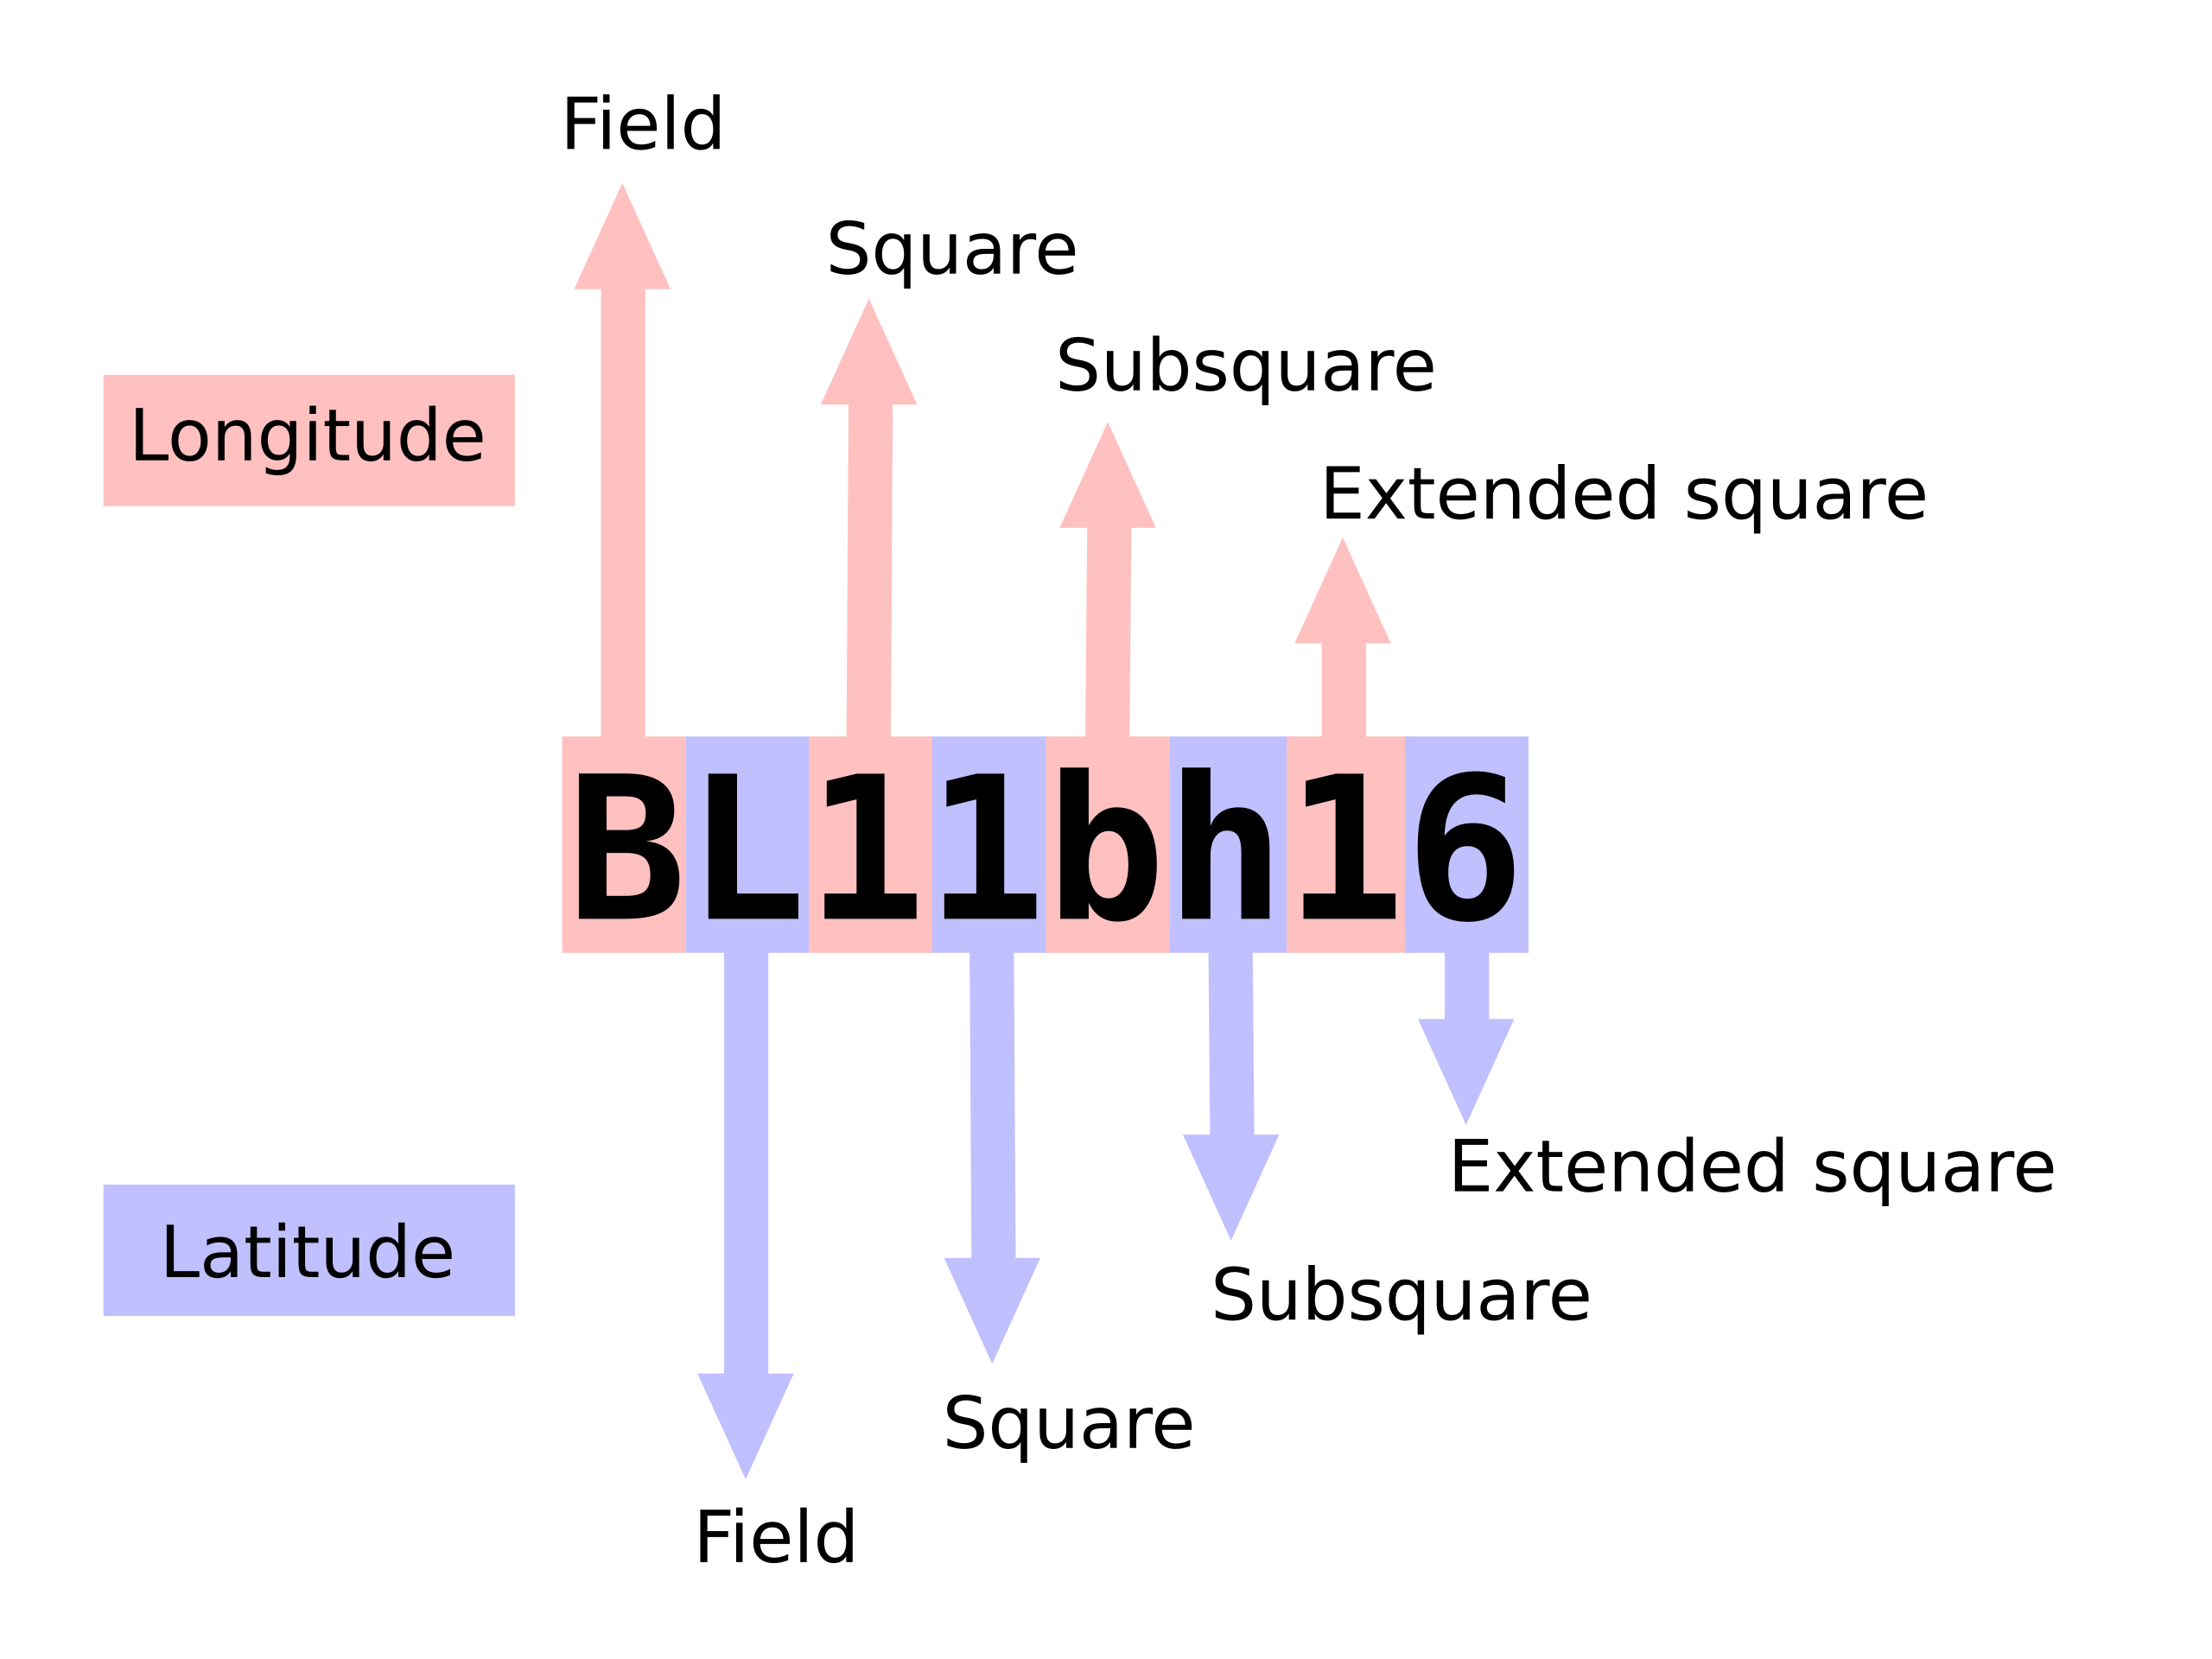
\includegraphics[width=0.5\textwidth]{pic/lokator.png}
	\caption{Lokatorns delar. Från Wikipedia.}
\end{figure}

Ett fält är ett stort geografiskt område så i regel pratar man om rutor och
använder mist de 4 första i lokatorn. Man är då nere på ungefär kommunnivå i
storlek.

Men oftast använder man också ''subsquare'' delen och är då nere på en ruta
som är en mindre tätort i storlek vilket är en ganska lagom stor yta. Min
lokator är t.ex. JP80TM.

\begin{figure}[H]
	\centering
	\subfloat{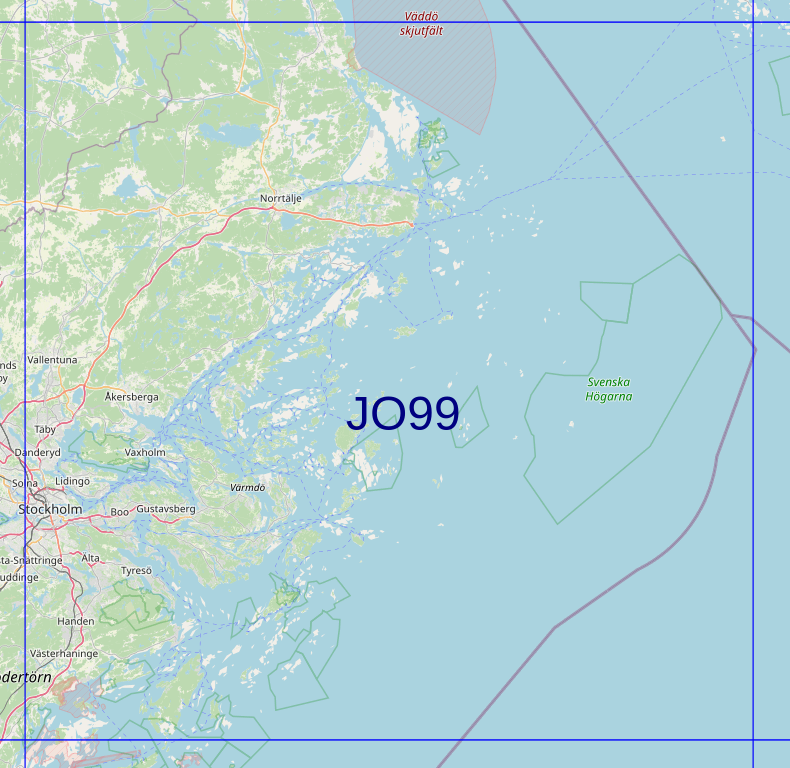
\includegraphics[width=0.35\textwidth]{pic/lokator-ruta.png}}%
	\qquad
	\subfloat{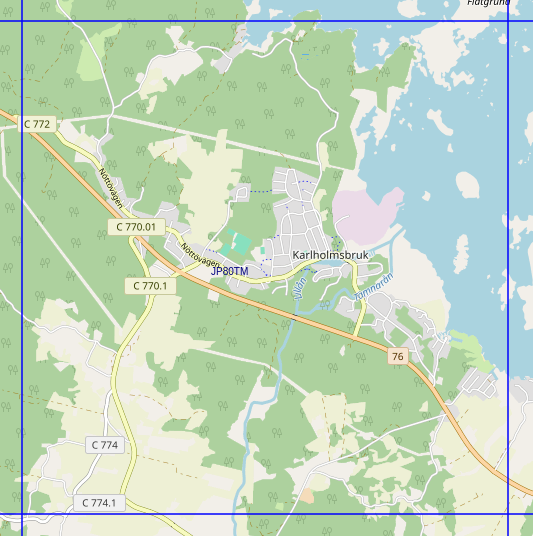
\includegraphics[width=0.35\textwidth]{pic/lokator-subruta.png}}
	\caption{Exempel på fyr- och sexställig lokator}
\end{figure}

Det finns många webresurser för att söka en lokator, en sådan är till exempel
denna som använder sig av Open Streetmaps,
\url{https://f5len.org/tools/locator} men det finns naturligtvis många andra
alternativ, inte minst som appar till telefoner och surfplattor.

\section{Missanpassning}

För maximal överföring av radioenergi från en sändare till en antenn eller
från antennen till en mottagare krävs att man har en bra anpassning mellan de
olika delarna. Dessa brukar vara tre saker som behöver "matchas" med varandra
så att man har en snarlik impedans hos alla tre.

Dessa är radioapparaten, transmissionsledningen och antennen. I de flesta fall
är radioapparaten en sändtagare som kan växla mellan sändning och mottagning.
Transmissionsledningen är vanligtvis någon form av koaxialkabel som har en så
kallad "karaktäristisk impedans" som i dessa sammanhang vanligtvis är
50\,$\Omega$.

\subsection{Stående våg}

Om anpassningen inte stämmer kommer man förlora energi på vägen och man får
ett felaktigt stående vågförhållande. På engelska kallas detta för Voltage
Standing Wave Ratio (spänningens ståendevågförhållande) och betecknas VSWR.
Det finns två vanligen förekommande sätt att mäta den och det ena är att man
mäter förhållandet mellan den framåtgående effekten och den reflekterade och
man betecknar dessa som ett bråktal, vanligen som 1:1,2.

\subsection{Return loss}

Man kan även uttrycka den i så kallad "return loss" eller RL. Detta begrepp
talar i stället om hur många decibel lägre den på grund av missanpassningen
reflekterade signalen är i förhållande till den framåtgående och utrycks i
decibel, vanligen som 20\,dB\,RL. Just denna siffra betyder att den
reflekterade signalen är 20\,dB lägre än den framåtgående signalen och det är
alltså 1\,\% som reflekteras.

\subsection{Bra och dålig anpassning}

En missanpassning kan sägas vara bra om den är bättre än 20\,dB\,RL och vi kan
säga att den är dålig om den är sämre än 10\,dB\,RL. I VSWR är det ungefär
1:1,2 och 1:2 ungefär.

\subsection{Konvertera mellan VSWR och RL}

\begin{equation}
	\text{RL} = 20 \cdot \log_{10} \frac{\text{VSWR}-1}{\text{VSWR}+1}
\end{equation}

\begin{equation}
	\text{VSWR} = \frac{1+10^\frac{\text{-RL}}{20}}{1-10^\frac{\text{-RL}}{20}}
\end{equation}

Där RL är return loss i dB och VSWR är ståendevågförhållandet, exempelvis 1,2.

\subsection{Tabell över stående våg och return loss}

\begin{table}[H]
\centering
\begin{tabular}{rr|rr|rr}
	\textbf{RL} & \textbf{VSWR} & \textbf{RL} & \textbf{VSWR} & \textbf{RL} & \textbf{VSWR} \\ \hline
	         40 &        1:1,02 &          18 &        1:1,29 &           8 &        1:2,32 \\
	         35 &        1:1,04 &          16 &        1:1,38 &           6 &        1:3,01 \\
	         30 &        1:1,07 &          14 &        1:1,50 &           4 &        1:4,42 \\
	         25 &        1:1,12 &          12 &        1:1,67 &           2 &        1:8,72 \\
	         20 &        1:1,22 &          10 &        1:1,92 &           1 &        1:17,4
\end{tabular}
\caption{Stående våg och return loss}
\label{tab:vswr-rl}
\end{table}

\section{Radioberäkningar för VHF och UHF}

Några av de vanligaste radioberäkningarna man kan komma att behöva göra.

\subsection{Beräkning av radiohorisonten}

Radiohorisonten är den sträcka som markvågen kan nå utan särskilda hjälpmedel
och i frånvaro av andra effekter som särskilda kondisioner (tropo eller
duktning) och liknande. Avståndet kan beräknas med hjälp av en enkel formel.
Radiohorisonten gäller egentligen bara när inget annat är i vägen men kan ge
en ledning till den längsta utbredning man kan förvänta sig med markvåg givet
en viss höjd.

För skepp på havet stämmer radiohorisonten ganska väl så man hittar denna
formel ofta i utbildningsmaterial för marin VHF men då med distansen i
nautiska mil i stället för km. För att få detta byter man konstanten 3,57 till
2,2 i stället.

\begin{equation}
	r = 3,57 \left(\sqrt{h_1}+\sqrt{h_2}\right)
\end{equation}

Där $r$ är avståndet till radiohorisonten givet i kilometer, $h_1$ är den ena
stationens antennhöjd över marken givet i meter och $h_2$ är den andra
stationens antennhöjd över marken också givet i meter.

Om motstationen befinner sig i markhöjd och det inte finns terräng som
blockerar kan man räkna ut hur lång din radiohorisont är på VHF-bandet baserat
enbart på din egen höjd med denna formel:

\begin{equation}
	r = \sqrt{17 \cdot h}
\end{equation}

För optisk sikt kan man säga följande:

\begin{equation}
	r = \sqrt{13 \cdot h}
\end{equation}

I båda ovanstående är radien $r$ i kilometer och höjden $h$ i meter.

\subsection{Sträckdämpning}

Sträckdämpningen beror på flera olika faktorer, inte minst terrängen och det
som finns mellan sändaren och mottagaren. I den fria rymden följer den en
enkel geometrisk utbredning men närmare marken behöver man stoppa in en del
kompensationsfaktorer.

\begin{equation}
	PL_0 = 20 \cdot \log(f) + 20 \cdot \log(d) - 27,55
\end{equation}

Där $PL_{0}$ är sträckdämpningen i decibel(dB) (Eng: Path Loss) mellan två
sändare givet avståndet $d$ i meter och frekvensen $f$ i MHz. Om man anger $d$
i kilometer i stället adderar man 60 till konstanten och får då 32,45.

För sträckdämpning vid mark får man mäta eller skatta en utbredningsdämpning
som en konstant $k$ som man använder för att modifiera formeln med och får då
följande variant:


\begin{equation}
	PL_m = 20 \cdot \log(f) + (20+k) \cdot \log(d) - 27,55
\end{equation}

Där $PL_m$ är sträckdämpningen vid marken. Faktorn $k$ kan uppskattas enligt
följande tabell:

\begin{table}[H]
	\begin{centering}
		\begin{tabular}{r|l}
			\textbf{k} & \textbf{Beskrivning} \\ \hline
			0 & Över öppen terräng med högre frekvenser och fri sikt\\
			5 & Lättare terräng, mindre kullar, gräs och få träd \\
			10 & Tuffare terräng med mer höjdvariation, klippblock, tätare skog \\
			15 & Urban miljö, större hus, höghus \\
			20 & Extremt urband miljö (tänk Manhattan)\\
		\end{tabular}
	\end{centering}
	\label{tab:frirum-faktor}
	\caption{Tabell över korrigeringsfaktor för frirumsutbredning vid marken}
\end{table}

I vanlig svensk terräng är det nog vanligast man hamnar i storleksordningen
5--10.


